\begin{frame}{The Landscape of Optimization}
    \framesubtitle{A Complex Surface}
    \small
    \begin{itemize}
        \item The error surface $E(W)$ for deep networks is extremely complex and \bhighlight{non-convex}. This means it's not a simple bowl shape, but rather a landscape filled with hills, valleys, and plateaus.
        \item This non-convexity introduces significant challenges for our gradient descent algorithm. The two main challenges are:
        \begin{itemize}
            \item \textbf{Local Minima:} Points that look like the bottom of a valley locally, but are not the true lowest point of the entire landscape.
            \item \textbf{Saddle Points:} Points where the gradient is zero, but they are not minima.
        \end{itemize}
    \end{itemize}
    \begin{figure}
        \centering
        % Source: Optimization I.pdf, Page: 4
        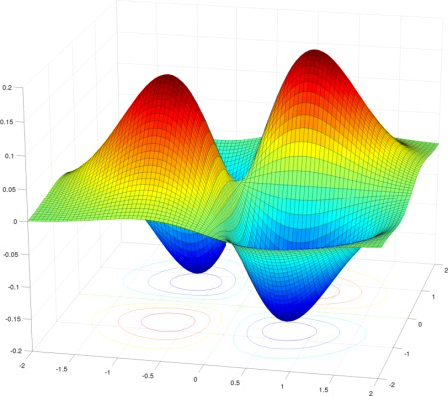
\includegraphics[width=0.3\linewidth]{images/error_surfaces.png}
        \caption{Examples of complex, non-convex error surfaces in neural networks.}
    \end{figure}
\end{frame}

\begin{frame}{The Landscape: Challenges}
    \framesubtitle{Saddle Points}
    \small
    \begin{itemize}
        \item A \bhighlight{saddle point} is a point where the gradient is zero, but it is a minimum along some dimensions and a maximum along others.
        \item Think of the shape of a horse's saddle: if you move forward or backward you go up, but if you move side to side you go down.
        \item For vanilla gradient descent, the gradient at a saddle point is zero (or very close to it), causing the algorithm to slow down dramatically or even get permanently "stuck".
    \end{itemize}
    \begin{figure}
        \centering
        % Source: Optimization I.pdf, Page: 3
        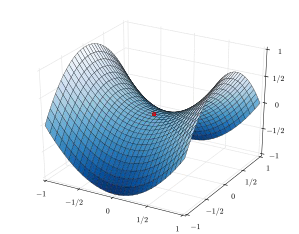
\includegraphics[width=0.5\linewidth]{images/saddle_point.png}
        \caption{A visualization of a saddle point. The gradient is zero at the center, but it is not a minimum.}
    \end{figure}
\end{frame}

\begin{frame}{The Landscape: Challenges}
    \framesubtitle{Saddle Points vs. Local Minima}
    \begin{itemize}
        \item A key insight in modern deep learning is that in very high-dimensional spaces (networks with many parameters), \bhighlight{saddle points are exponentially more common} than local minima.
        \item For a point to be a local minimum, the curvature must be positive in \emph{all} dimensions. The probability of this happening simultaneously in millions of dimensions is extremely small.
        \item This is actually good news! It means that most of the points with zero gradient that our optimizer finds are saddle points, which advanced optimizers (like those with momentum) are better at escaping, rather than "bad" local minima that would permanently trap the algorithm.
    \end{itemize}
\end{frame}